\documentclass[12pt,]{article}
\usepackage{lmodern}
\usepackage{amssymb,amsmath}
\usepackage{ifxetex,ifluatex}
\usepackage{fixltx2e} % provides \textsubscript
\ifnum 0\ifxetex 1\fi\ifluatex 1\fi=0 % if pdftex
  \usepackage[T1]{fontenc}
  \usepackage[utf8]{inputenc}
\else % if luatex or xelatex
  \ifxetex
    \usepackage{mathspec}
  \else
    \usepackage{fontspec}
  \fi
  \defaultfontfeatures{Ligatures=TeX,Scale=MatchLowercase}
    \setmainfont[]{Times New Roman}
\fi
% use upquote if available, for straight quotes in verbatim environments
\IfFileExists{upquote.sty}{\usepackage{upquote}}{}
% use microtype if available
\IfFileExists{microtype.sty}{%
\usepackage{microtype}
\UseMicrotypeSet[protrusion]{basicmath} % disable protrusion for tt fonts
}{}
\usepackage[margin=2.54cm]{geometry}
\usepackage{hyperref}
\hypersetup{unicode=true,
            pdftitle={A Case Study on Chemical Flashiness of Streams and Canals in Florida},
            pdfauthor={Ethan Ready, Gabi Richichi, Theo Cai, Yutao Gong},
            pdfborder={0 0 0},
            breaklinks=true}
\urlstyle{same}  % don't use monospace font for urls
\usepackage{longtable,booktabs}
\usepackage{graphicx,grffile}
\makeatletter
\def\maxwidth{\ifdim\Gin@nat@width>\linewidth\linewidth\else\Gin@nat@width\fi}
\def\maxheight{\ifdim\Gin@nat@height>\textheight\textheight\else\Gin@nat@height\fi}
\makeatother
% Scale images if necessary, so that they will not overflow the page
% margins by default, and it is still possible to overwrite the defaults
% using explicit options in \includegraphics[width, height, ...]{}
\setkeys{Gin}{width=\maxwidth,height=\maxheight,keepaspectratio}
\IfFileExists{parskip.sty}{%
\usepackage{parskip}
}{% else
\setlength{\parindent}{0pt}
\setlength{\parskip}{6pt plus 2pt minus 1pt}
}
\setlength{\emergencystretch}{3em}  % prevent overfull lines
\providecommand{\tightlist}{%
  \setlength{\itemsep}{0pt}\setlength{\parskip}{0pt}}
\setcounter{secnumdepth}{5}
% Redefines (sub)paragraphs to behave more like sections
\ifx\paragraph\undefined\else
\let\oldparagraph\paragraph
\renewcommand{\paragraph}[1]{\oldparagraph{#1}\mbox{}}
\fi
\ifx\subparagraph\undefined\else
\let\oldsubparagraph\subparagraph
\renewcommand{\subparagraph}[1]{\oldsubparagraph{#1}\mbox{}}
\fi

%%% Use protect on footnotes to avoid problems with footnotes in titles
\let\rmarkdownfootnote\footnote%
\def\footnote{\protect\rmarkdownfootnote}

%%% Change title format to be more compact
\usepackage{titling}

% Create subtitle command for use in maketitle
\providecommand{\subtitle}[1]{
  \posttitle{
    \begin{center}\large#1\end{center}
    }
}

\setlength{\droptitle}{-2em}

  \title{A Case Study on Chemical Flashiness of Streams and Canals in Florida}
    \pretitle{\vspace{\droptitle}\centering\huge}
  \posttitle{\par}
  \subtitle{\url{https://github.com/ytgong/ENV322_group_project}}
  \author{Ethan Ready, Gabi Richichi, Theo Cai, Yutao Gong}
    \preauthor{\centering\large\emph}
  \postauthor{\par}
    \date{}
    \predate{}\postdate{}
  
\usepackage{float}
\floatplacement{figure}{H}

\begin{document}
\maketitle

\newpage

\hypertarget{rationale-and-research-questions}{%
\section{Rationale and Research
Questions}\label{rationale-and-research-questions}}

\hypertarget{rationale}{%
\subsection{Rationale}\label{rationale}}

Storm events have the potential to influence rivers and streams by
temporarily altering their discharge levels and chemical composition.
Rapid changes in stream discharge is known as hydrologic flashiness (1).
A stream that ``experiences a rapid increase in flow shortly after onset
of a precipitation event, and an equally rapid return to base conditions
shortly after the end of the precipitation event'' is considered to be
hydrologically ``flashy'' (1). Rapid changes in chemical composition,
such as nutrient concentrations or conductance levels, is known as
chemical flashiness or a departure from chemostasis. ``Chemostasis
occurs when DOM {[}dissolved organic matter{]} remains unchanged despite
changes in discharge'' (2).

Both hydrologic and chemical flashiness can alter the natural processes
of rivers and streams, particularly if these rivers and streams are
experiencing an increase in flashiness over time. These alterations can
disrupt human activity such as hunting, fishing, recreation, and the
utilization of water for drinking, and, as a result, people incur costs.
One consequence of hydrologic flashiness is flooding of nearby lands.
Flooding events in the U.S. cost an average of 4.4 billion USD per event
in damages (5). One alteration caused by storm-induced flashiness is
eutrophication. Eutrophication ``is characterized by excessive plant and
algal growth due to the increased availability of one or more limiting
growth factors needed for photosynthesis, such as sunlight, carbon
dioxide, and nutrient fertilizers'' (6). In this case, the limiting
growth factor that chemical flashiness can increase is nutrient levels.
As nutrient levels increase, this can cause ``blooms of blue-green
algae(i.e., cyanobacteria), tainted drinking water supplies, degradation
of recreational opportunities, and hypoxia. The estimated cost of damage
mediated by eutrophication in the U.S. alone is approximately \$2.2
billion annually'' (7).

The effects of storm events on bodies of water are compounded by human
activity. The use of pesticides and fertilizers on agricultural land, as
well as the way in which sewage is managed, can make nutrients such as
nitrogen and phosphorus accessible for storm transport in the first
place (8). Furthermore, anthropogenically-induced climate change is
intensifying natural precipitation events by making them wetter, longer,
and more intense (9). As storms worsen, so do their effects.

This applies to the region of this study in particular. Florida is a
state that has a history of extreme weather events such as hurricanes
and tropical storms, as well as a history, particularly recently, of
eutrophication events. High levels of nutrient loading, in combination
with high temperatures that are typical of Florida's climate, create an
environment conducive to eutrophication (5). The Florida Department of
Environmental Protection lists more than 1,400 water bodies as
``impaired by pollutants'' (5). In this study, 21 water bodies including
rivers, creeks, springs, and canals in Florida are examined for their
hydrologic and chemical flashiness, the urbanness or ruralness of their
surrounding lands, as well as the water use levels of the surrounding
communities.

These sites are of great importance to people. For example,
Chassahowitzka River is a spring-fed river in a national wildlife
refuge, on which people engage in sportfishing, crabbing, camping, and
hiking activities (6). The Main Relief Canal in Vero Beach, managed by
the Indian River Farms Water Control District, drains much of Indian
River County and the City of Vero Beach to prevent flooding on
residential and commercial land (10). Turnbull Creek is a ``critical
waypoint for waters flowing north into Turnbull Bay, Spruce Creek, the
Indian River, and Atlantic Ocean'' (11) and a habitat for numerous
species (12). A majority of the people of New Smyrna Beach (75\% of
constituents) just voted in favor of a referendum to pay \$8.94 million
to protect the land along Turnbull Creek from development (13). Many of
the sites of this study are well-managed, located in state or national
parks, and all of the canals are artificially created. There are already
management-schemes and policies in place to protect these water bodies.
For example, to reduce nutrient total maximum daily loads, there exists
action plans (14) and the Springs Protection Act (15). It is useful,
then, to better understand the effects of flashiness on these water
bodies in order to inform managers to implement more efficient and
cost-effective management practices.

\hypertarget{research-questions}{%
\subsection{Research Questions}\label{research-questions}}

The goal of this study was to better understand the effects of storm
events on rivers and streams in Florida. The following questions and
hypotheses guided the study: Question 1: Is there a correlation between
hydrologic and chemical flashiness in rivers and streams?

Hypothesis 1: There is a correlation between hydrologic and chemical
flashiness. Sites with high hydrologic flashiness are more likely to be
chemically flashy because of shared predictor variables.

Question 2: How do rural / urban features of a site impact its chemical
flashiness?

Hypothesis 2: There is a correlation between the urbanness / ruralness
of a site and its chemical flashiness. Sites with high urbanness are
more likely to be chemically flashy because of impervious surfaces and
non-point source discharge potential.

\newpage

\hypertarget{dataset-information}{%
\section{Dataset Information}\label{dataset-information}}

Data for 21 water bodies (7 rivers, 7 springs, 3 creeks, and 4 canals)
in Florida will be collected.

For question / hypothesis 1 regarding hydrologic and chemical
flashiness, high frequency discharge and nitrate data will be extracted
from the USGS NWIS DataRetrieval package. A Richards-Baker Index will be
calculated using the discharge data as a measure of hydrologic
flashiness. C-Q plots will be generated using the nitrate data as a
measure of chemical flashiness.

For question / hypothesis 2 regarding the properties of each site that
may affect chemical flashiness, data will be retrieved from United
States Geological Survey (USGS). Specifically, county population values,
irrigation water use levels, thermoelectric water use levels, and a
chemostatic coefficient will be examined. Maps taken from ArcGIS will be
examined to ascertain the presence or absence of features indicative of
urbanness or ruralness surrounding each site, such as airports,
commercial center, or farms, as well as the proximity of these features
to each water body.

\begin{longtable}[]{@{}lll@{}}
\caption{Variables used for analysis}\tabularnewline
\toprule
Variable & Units & Type\tabularnewline
\midrule
\endfirsthead
\toprule
Variable & Units & Type\tabularnewline
\midrule
\endhead
Nitrate concentrations -- high frequency & ng/L &
Independent\tabularnewline
Discharge -- high frequency & m\^{}3/s & Independent\tabularnewline
Richards-Baker Index value & & Independent\tabularnewline
County population & k people & Independent\tabularnewline
Irrigation water use & Bgal/day & Independent\tabularnewline
Thermoelectric water use & Bgal/day & Independent\tabularnewline
Chemostatic coefficient & & Dependent\tabularnewline
\bottomrule
\end{longtable}

\begin{longtable}[]{@{}rlll@{}}
\caption{USGS sites selected for analysis}\tabularnewline
\toprule
Site No. & Station Name & County & Abbr.\tabularnewline
\midrule
\endfirsthead
\toprule
Site No. & Station Name & County & Abbr.\tabularnewline
\midrule
\endhead
2326526 & WACISSA RIVER NR WACISSA FLA & Jefferson & WAC\tabularnewline
2319302 & MADISON BLUE SPRING NR BLUE SPRINGS, FL & Madison &
MAD\tabularnewline
2319950 & BLUE SPRINGS NEAR DELL,FL & Lafayette & BLUE\tabularnewline
2323566 & MANATEE SPRING NR CHIEFLAND FLA & Levy & MAN\tabularnewline
2323502 & FANNING SPRINGS NR WILCOX FLA & Levy & FAN\tabularnewline
2322800 & SANTA FE RIVER NR HILDRETH FLA & Gilchrist &
SANTA\tabularnewline
2322700 & ICHETUCKNEE R @ HWY27 NR HILDRETH, FL & Columbia &
ICHE\tabularnewline
2322688 & BLUE HOLE SPRING NR HILDRETH, FL & Columbia &
HOL\tabularnewline
2310743 & HUNTER SPR RUN AT BEACH LANE AT CRYSTAL RIVER FL & Citrus &
HUN\tabularnewline
2310678 & HOMOSASSA SPRINGS AT HOMOSASSA SPRINGS FL & Citrus &
HOM\tabularnewline
2310650 & CHASSAHOWITZKA RIVER NEAR HOMOSASSA FL & Citrus &
CHAS\tabularnewline
2313100 & RAINBOW RIVER AT DUNNELLON, FL & Marion & RAIN\tabularnewline
2313098 & RAINBOW RIVER NEAR DUNNELLON, FL & Marion & BOW\tabularnewline
2292900 & CALOOSAHATCHEE RIVER AT S-79, NR.OLGA, FLA & Lee &
CAL\tabularnewline
2289035 & THREE MILE CANAL BELOW G409 NEAR CLEWISTON, FL & Hendry &
THREE\tabularnewline
2248350 & TURNBULL CREEK NR OAK HILL, FL & Volusia & TURN\tabularnewline
2248600 & DRAINAGE CANAL AT PLAZA PKWY AT COCOA, FL & Brevard &
DRAIN\tabularnewline
2249500 & CRANE CREEK AT MELBOURNE, FL & Brevard & CRANE\tabularnewline
2250030 & TURKEY CREEK AT PALM BAY, FL & Brevard & TURK\tabularnewline
2251767 & FELLSMERE CANAL NEAR MICCO, FL & Brevard & FELL\tabularnewline
2253000 & MAIN CANAL AT VERO BEACH, FL & Indian River &
MAIN\tabularnewline
\bottomrule
\end{longtable}

\newpage

\hypertarget{exploratory-analysis}{%
\section{Exploratory Analysis}\label{exploratory-analysis}}

Figure 1 is a map that shows the watershed and water feature information
of Florida and location of the sites we chose to analyze. It can be seen
that the sites chosen encompass a variety of water features, ranging
from streams, banks, to canals. They are also located in different
regions of Florida, and the hydrological heterogeneity among sites
offers an opportunity to study the potentially different interactions
between chemostaticity and hydrological flashiness.

\begin{figure}

{\centering 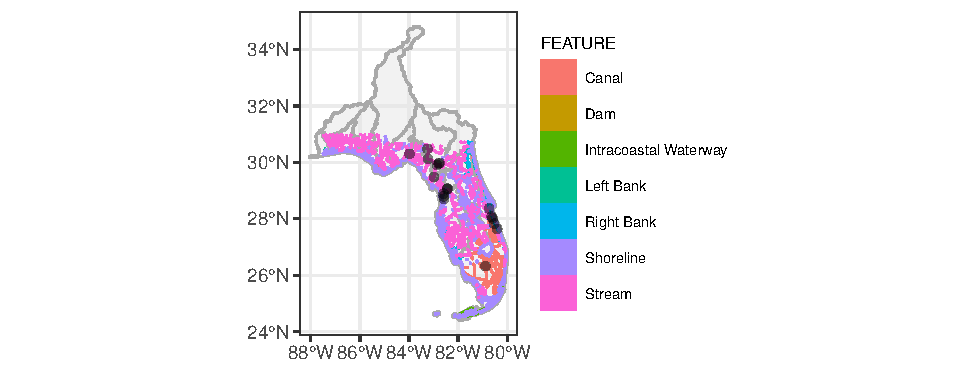
\includegraphics{Final-Project-Report_files/figure-latex/unnamed-chunk-3-1} 

}

\caption{Location of sites analyzed on watersheds}\label{fig:unnamed-chunk-3}
\end{figure}

We used violin plots to visualize the ranges of discharge and nitrate in
the different sites. We made individual violin plots for discharge and
nitrate for each site, and noticed the difference between the canal
plots and the other waterway types (Figure 2). The canal plots have
values much more concentrated in their lower ranges, and much less
variation overall. Visualizing the differences in canal variable
distributions alerts us that they may influence our data analysis.

\begin{figure}
\centering
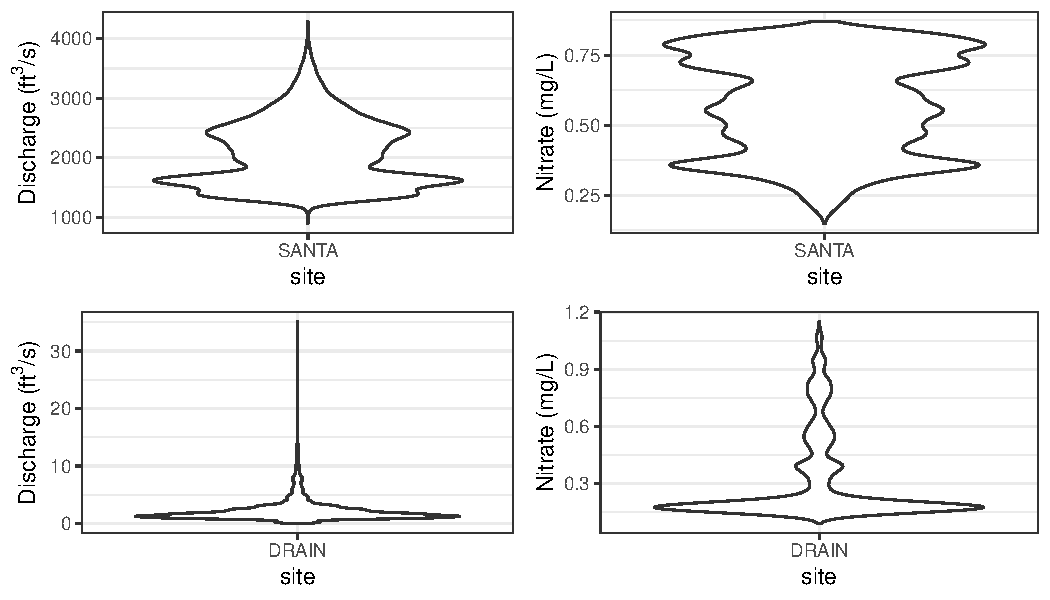
\includegraphics{Final-Project-Report_files/figure-latex/unnamed-chunk-4-1.pdf}
\caption{Distribution of discharge and nitrate values of a stream and a
canal}
\end{figure}

We then created combined violin plots of discharge and nitrate for all
the sites. The CAL and SANTA sites had much more discharge than any
other site so here we present the discharge plot without CAL and SANTA
to better visualize the smaller discharges (Figure 3). A similar plot
for nitrate was also made (Figure 4).

\begin{figure}
\centering
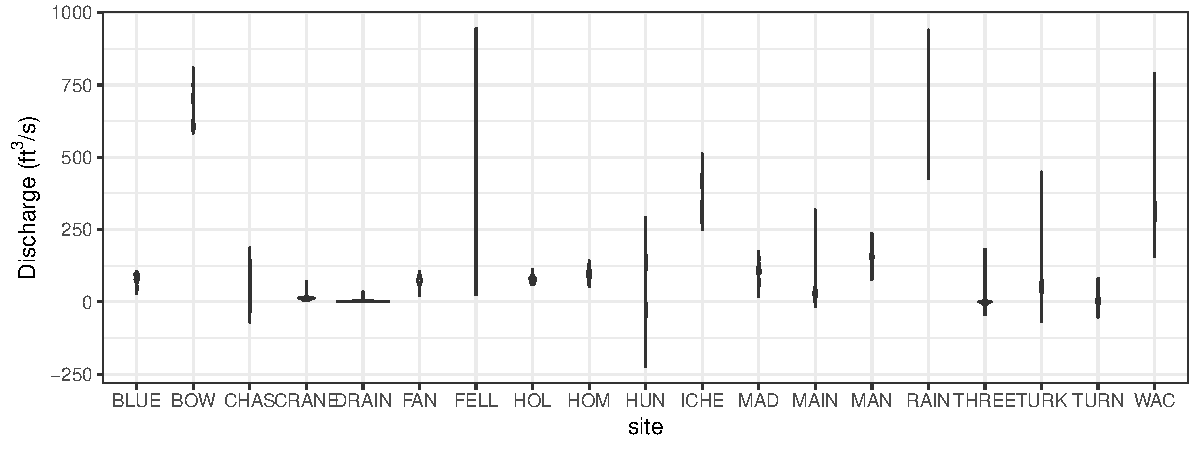
\includegraphics{Final-Project-Report_files/figure-latex/unnamed-chunk-5-1.pdf}
\caption{Distribution of discharge values of all sites (except CAL and
SANTA)}
\end{figure}

\begin{figure}
\centering
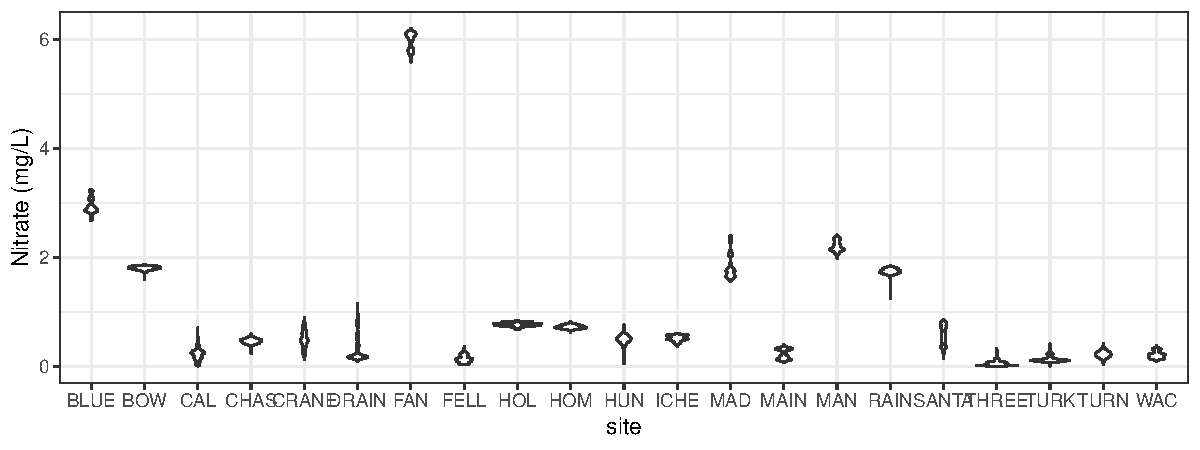
\includegraphics{Final-Project-Report_files/figure-latex/unnamed-chunk-6-1.pdf}
\caption{Distribution of nitrate concentration values of all sites}
\end{figure}

Our final exploratory analysis consisted of plotting discharge and
nitrate over time at all 21 of our sites. This served two purposes: one,
it helped us get a preliminary sense of the diversity in distributions
and behaviors at all of the sites, and two, it highlighted any possible
gaps in the data that we would need to wrangle out. In general, we did
not notice any trends between sites, indicating a deeper analysis was
needed.

This report includes four examples of the graphs we generated: one
spring, one river, one canal, and one creek (Figure 5) - all to give a
sense of the range of site types and the data trends at each.

\begin{figure}
\centering
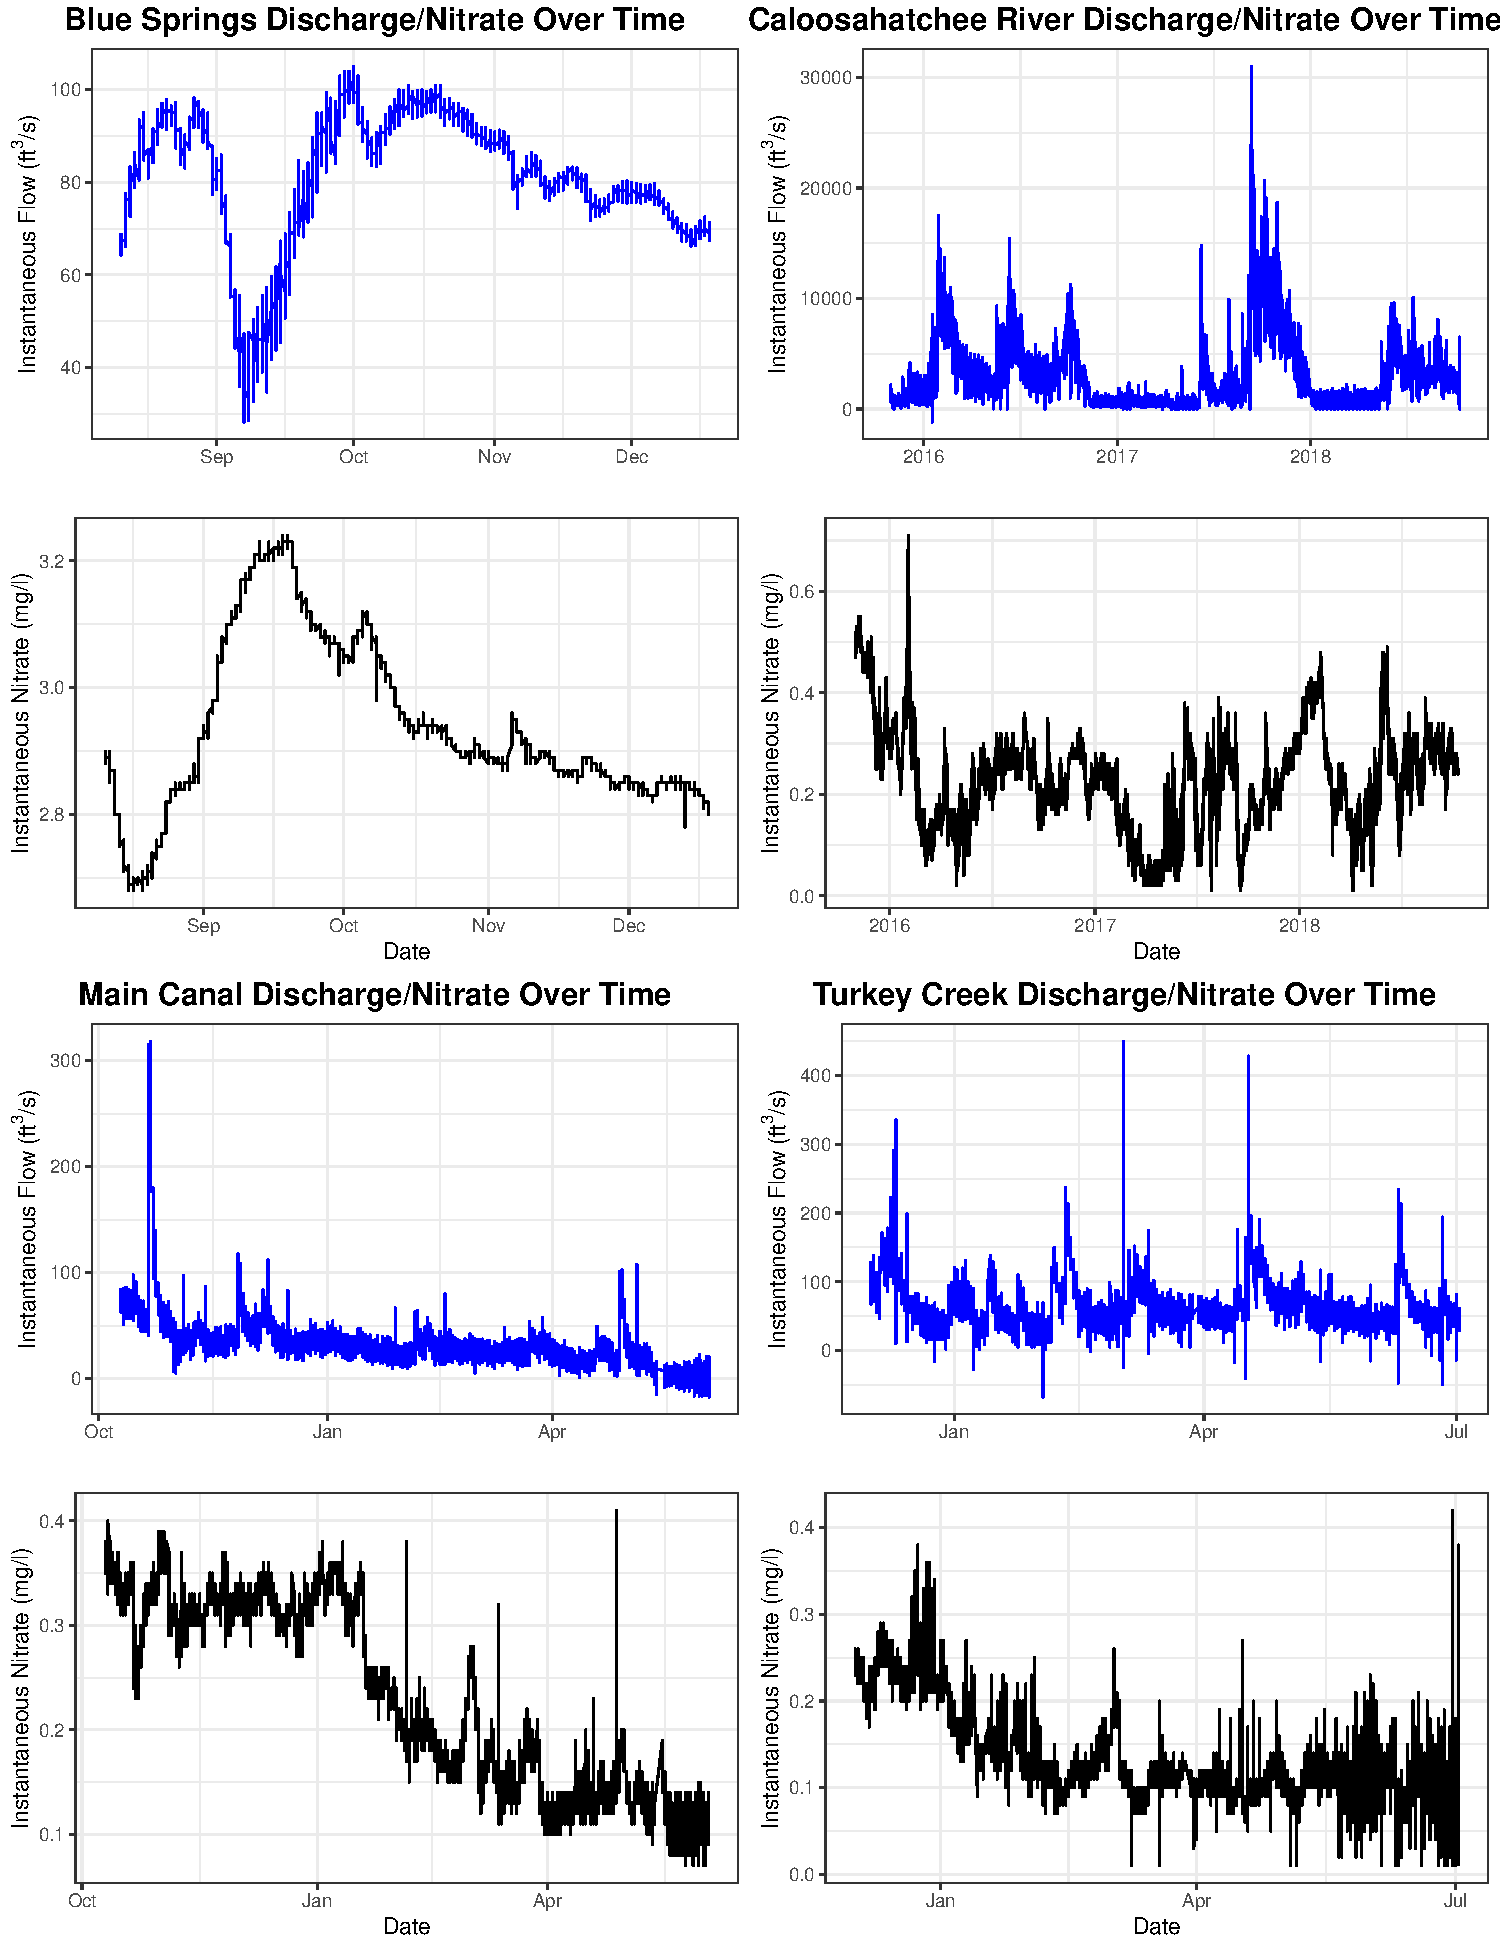
\includegraphics{Final-Project-Report_files/figure-latex/unnamed-chunk-7-1.pdf}
\caption{Discharge and nitrate value patterns of example sites}
\end{figure}

\newpage

\hypertarget{analysis}{%
\section{Analysis}\label{analysis}}

\hypertarget{question-1-are-sites-with-high-hydrologic-flashiness-more-or-less-likely-to-have-high-chemical-flashiness}{%
\subsection{Question 1: Are sites with high hydrologic flashiness more
or less likely to have high chemical
flashiness?}\label{question-1-are-sites-with-high-hydrologic-flashiness-more-or-less-likely-to-have-high-chemical-flashiness}}

We chose to analyze our first question, on the relationship between
hydrologic flashiness and chemical flashiness, using sites with high
frequency nitrate and discharge measurements. At each site, we
calculated the Richards-Baker Index to quantify the hydrologic
flashiness. We had to exclude catchment size in the formula because 17
out of 21 sites did not have a recorded catchment size.

To quantify chemical flashiness, we ran a linear regression between mean
daily nitrate and mean daily discharge values and took the coefficient
as our chemostaticity value. We excluded 3 sites with poor linear
regression fits, 1 of which had a large outlier for chemostaticity
coefficient.

We wrangled the RBI values and Chemostaticity Coefficients to create a
dataframe with columns site, site type (canal, river, etc.),
chemostaticity coefficient, chemostaticity coefficient absolute value,
and RBI value. We included the absolute value of the Chemostaticity
Coefficient to investigate the flashiness, as absolute value would
account for large chemostaticity in either a flushing or diluting
system.

We created ggplot visualizations of Chemostatic Coefficient vs.~RBI
(Figure 6) and Absolute Chemostatic Coefficient vs.~RBI (Figure 7)
separating site type by color. The visualization without absolute value
shows a distribution that follows the x and y axis. Sites with large RBI
values have low Chemostatic Coefficients, and sites with low RBI values
have Chemostatic Coefficients that are far above 0 or far below 0. The
absolute value visualization reinforces this finding, as large absolute
Chemostatic Coefficients correspond with small RBI values. Similar
trends were viewed between site type, except that the largest outlier
for both Chemostatic Coefficient and RBI are both canals.

\begin{figure}
\centering
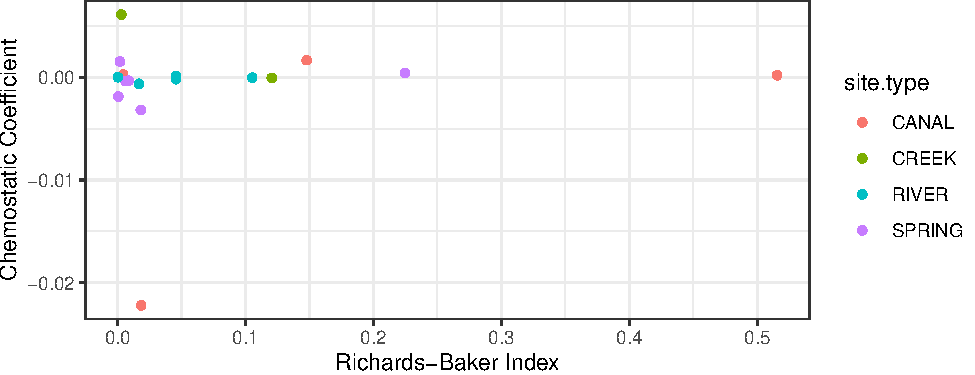
\includegraphics{Final-Project-Report_files/figure-latex/unnamed-chunk-9-1.pdf}
\caption{Chemostatic coefficient values and Richards-Baker Index of 18
sites}
\end{figure}

\begin{figure}
\centering
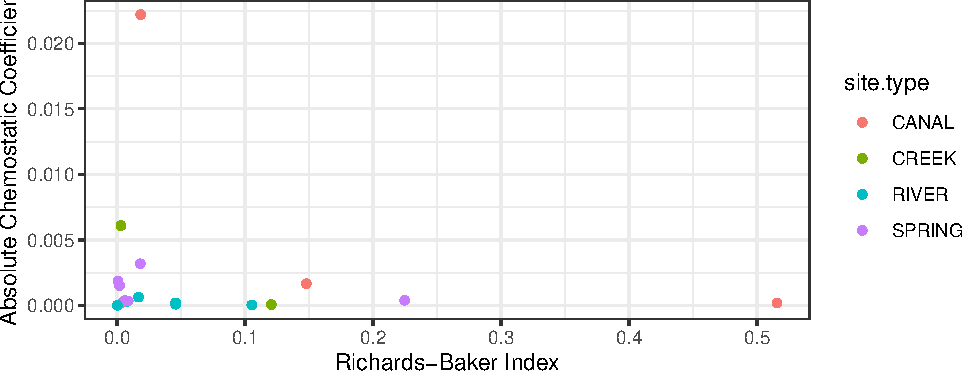
\includegraphics{Final-Project-Report_files/figure-latex/unnamed-chunk-10-1.pdf}
\caption{Absolute Chemostatic coefficient values and Richards-Baker
Index of 18 sites}
\end{figure}

We ran a linear regression on log(Absolute Chemostatic Coefficient)
vs.~RBI, which was the closest fit that we could find. The regression
produced a coefficient of -2.6847 , a P-value of 0.473, and a multiple
r-squared of 0.03264. The model does not adequately predict the data.

Since canals often act differently than natural waterways, and the
largest outlier for both RBI and Chemostaticity Coefficient are canals,
we also visualized the data without canals (Figure 8). The
visualizations are more clear due to smaller axis ranges, and show
similar results to the first visualizations. We ran the same linear
regression on the Absolute Chemostatic Coefficient without canals.

\begin{figure}
\centering
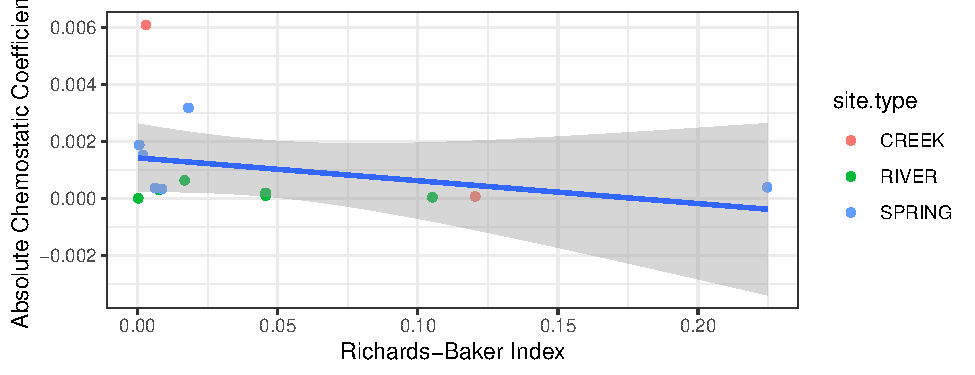
\includegraphics{Final-Project-Report_files/figure-latex/unnamed-chunk-12-1.pdf}
\caption{Absolute Chemostatic coefficient values and Richards-Baker
Index of 14 non-canal sites}
\end{figure}

The linear regression for Absolute Chemostatic Coefficient vs.~RBI
provided a Coefficient of -6.889, a P-value of 0.39, and a multiple
r-squared of 0.06228. While the fit doesn't sufficiently match the data,
it is better than the data with canals and does provide some idea of the
relationship between the variables.

\hypertarget{question-2-how-do-features-of-a-site-impact-its-chemical-flashiness}{%
\subsection{Question 2: How do features of a site impact its chemical
flashiness?}\label{question-2-how-do-features-of-a-site-impact-its-chemical-flashiness}}

\hypertarget{qualitative-approach-how-do-geographical-features-impact-the-sites-chemical-flashiness}{%
\subsubsection{Qualitative Approach: How do geographical features impact
the site's chemical
flashiness?}\label{qualitative-approach-how-do-geographical-features-impact-the-sites-chemical-flashiness}}

We made observations by first sorting sites into three categories -
Chemostatic, Flushing, and Diluting - based on the slopes of the
regression lines of their C-Q plots - values near 0, positive values,
and negative values, respectively. Then, we went site by site and
searched their coordinates into Google Maps and ArcGIS, and noted the
general surrounding geography - is it mostly urban or rural? Is it in a
state park, adjacent to it, or nowhere near? Where, generally, in
Florida is this site located? We also paid special attention to the site
type - river, spring, or canal - as each most likely have differing
management strategies and hydrologies.

When we were done listing the qualitative traits of all the sites in
each hydrologic behavioral categorical, we noticed some trends had
emerged. For the most flushing sites, or, the ones with the steepest
regression line slopes, we noticed that all are located near airports.
(Main Canal, Fellsmere Canal, Crane Creek, and Madison Blue Spring)
There does not seem to be a correlation with the urbanity of the
location, however, as two out of four of these sites are mostly rural
and two are mostly urban - Fellsmere, Madison Blue Spring and Main
Canal, Crane Creek, respectively. We hesitate to draw any concrete
conclusions about possible relationships between flushing systems and
proximity to airports, as there may be many other factors involved that
are not within the scope of this project. One important factor could be
the management style of the site; three out of four of the canals
analyzed in this project tend towards flushing. This, too, could be a
coincidence, and we would need to do a deeper analysis with more sites
to draw conclusions.

Our list of diluting sites show more convincing trends - seven out of
nine of the sites are located in very rural locations, most in or on the
edge of a Florida state park. (Ichetucknee, Santa Fe, Blue Spring, Blue
Hole Spring, Manatee Spring, Homosassa Spring, Turkey Creek) However,
this number may be slightly inflated because three of the four most
diluting sites are directly interconnected, increasing the likelihood of
similar hydrologic tendencies between them. (Ichetucknee, Santa Fe, Blue
Hole Spring) There seem to be no other notable qualitative trends for
diluting sites.

Chemostatic or mostly chemostatic systems do not seem to display any
particular kind of trend. They are located in all kinds of environments
- from hyper-urban to deep in state parks.

\begin{figure}
\centering
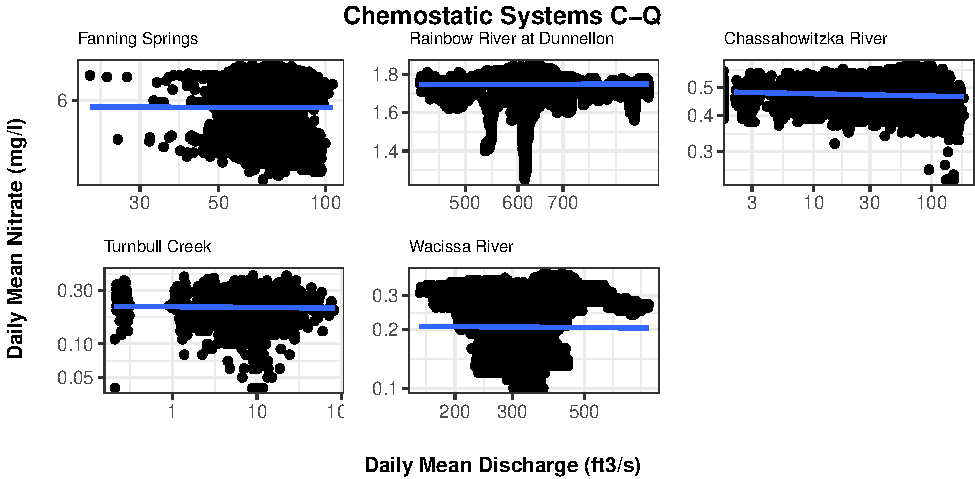
\includegraphics{Final-Project-Report_files/figure-latex/unnamed-chunk-14-1.pdf}
\caption{C-Q Plots of Chemostatic Sites}
\end{figure}

\begin{figure}
\centering
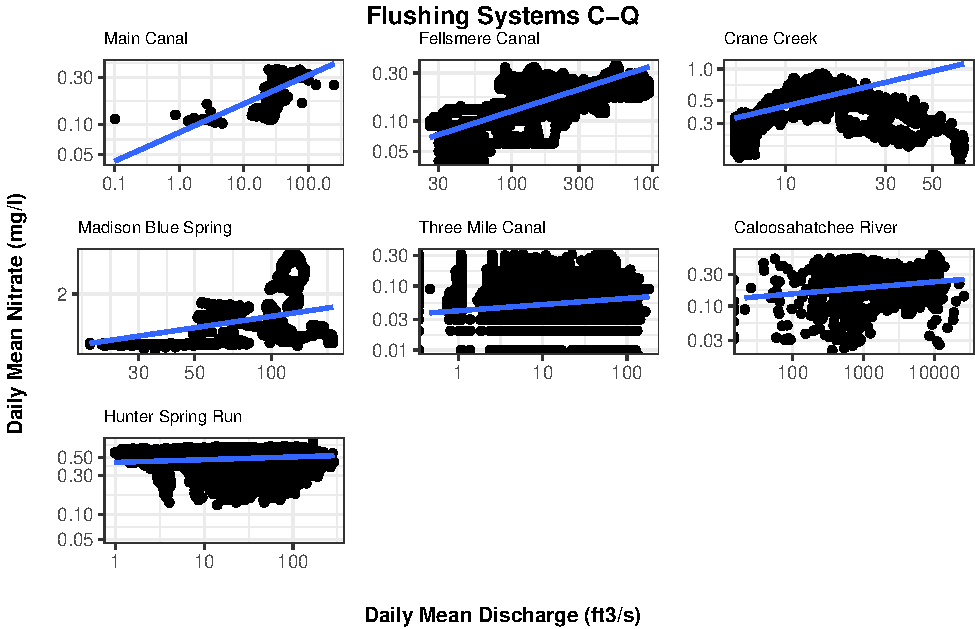
\includegraphics{Final-Project-Report_files/figure-latex/unnamed-chunk-15-1.pdf}
\caption{C-Q Plots of Flushing Sites}
\end{figure}

\begin{figure}
\centering
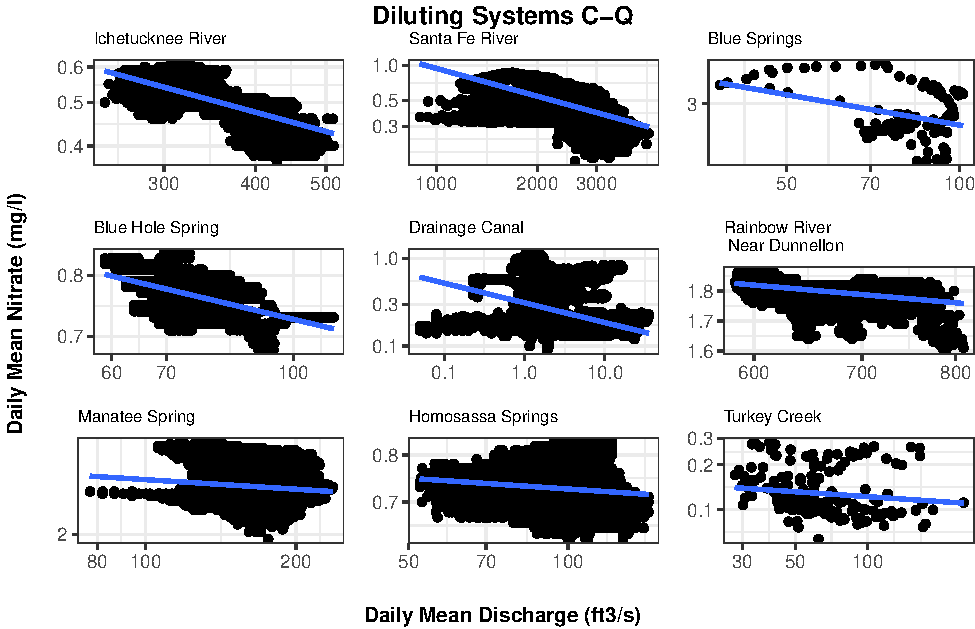
\includegraphics{Final-Project-Report_files/figure-latex/unnamed-chunk-16-1.pdf}
\caption{C-Q Plots of Diluting Sites}
\end{figure}

\hypertarget{quantitativestatistical-approach-how-do-counties-population-and-water-usage-impact-the-chemical-flashiness-of-sites-within-the-county}{%
\subsubsection{Quantitative/Statistical Approach: How do counties'
population and water usage impact the chemical flashiness of sites
within the
county?}\label{quantitativestatistical-approach-how-do-counties-population-and-water-usage-impact-the-chemical-flashiness-of-sites-within-the-county}}

Figure 12 shows each site's chemostaticity (absolute chemostatic
coefficient) on the water feature map. Based on the map, it appears that
sites on the right bank are less chemostatic, compared to sites in
central-northern part of Florida. However, since many factors are
confounding and sample size is not big enough, no definite conclusion
can be drawn.

\begin{figure}
\centering
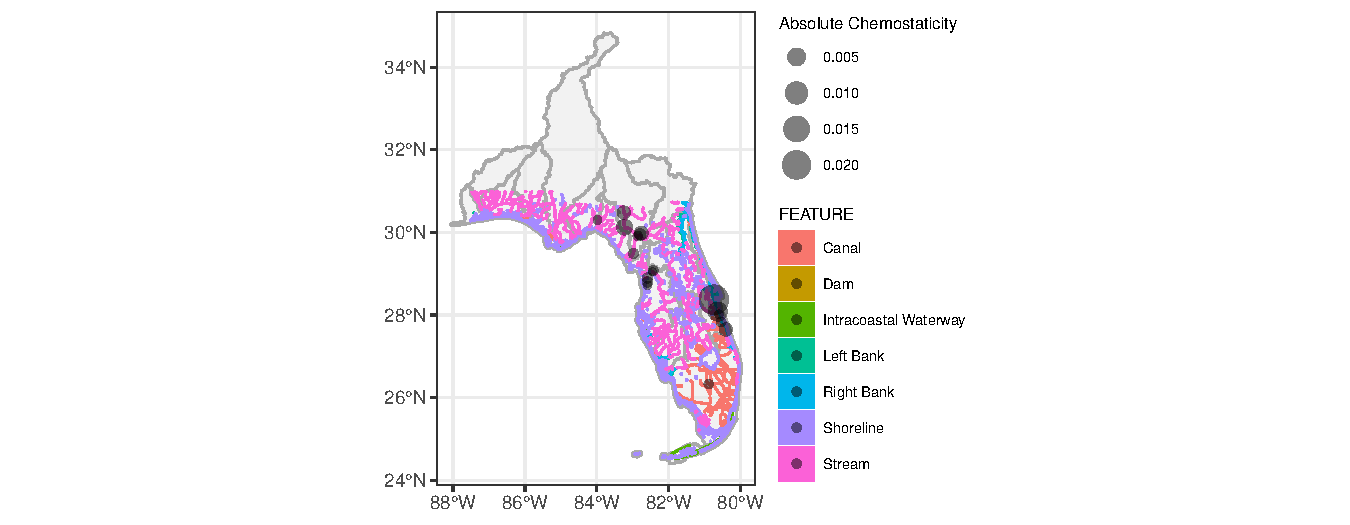
\includegraphics{Final-Project-Report_files/figure-latex/unnamed-chunk-17-1.pdf}
\caption{Location of sites and respective absolute chemostatic
coefficient}
\end{figure}

We then used county population and water use data from USGS to conduct a
quantitative analysis on how sites in different locations have different
levels of chemical flashiness. Specifically, for water use, we looked at
billion gallons of water used per day for irrigation and thermo
electricity generation in each county. We believe that the more water
used for irrigation in a county, the higher probability the sites in
that county have of being influenced by nutrient run-off from farms
within the county. A large amount of water used for thermo electricity
generation may either imply that the water is well-managed and therefore
more chemically stable, or imply that pollution may come from the
generation process and make the water chemically flashy.

Figure 13 shows that sites in counties with higher population seem to
have a higher probability of having higher absolute chemostatic
coefficient, which means that they are less chemically stable. However,
relationship between water use and chemical flashiness is not convincing
enough.

\begin{figure}
\centering
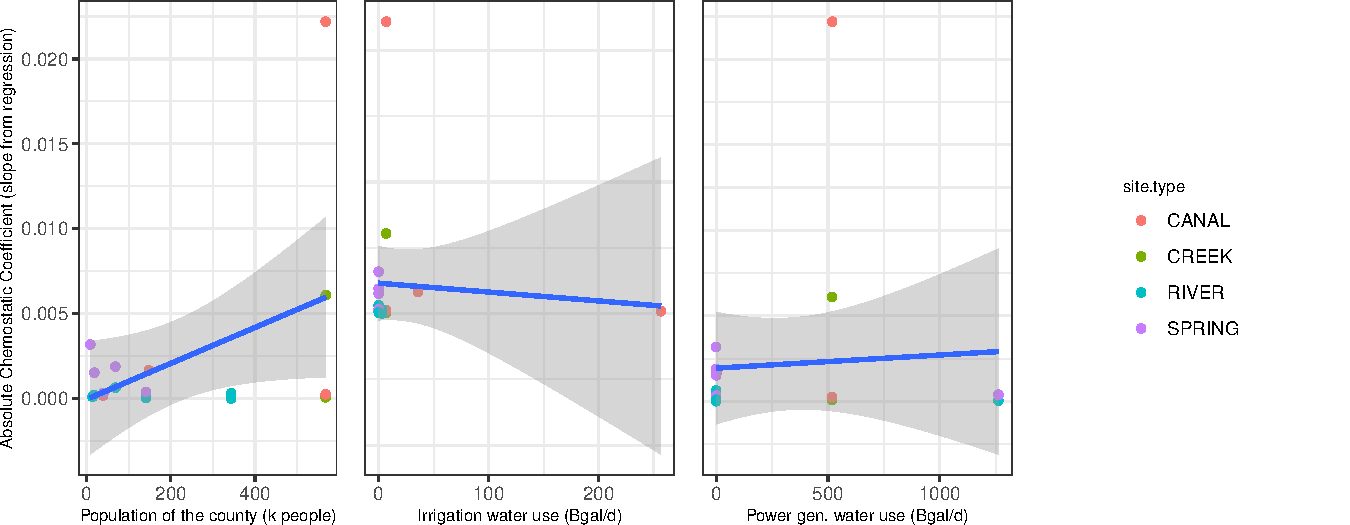
\includegraphics{Final-Project-Report_files/figure-latex/unnamed-chunk-18-1.pdf}
\caption{Relationship between a site's chemical flashiness and
population and water use of the county the site is in}
\end{figure}

We ran a linear regression to quantify the relationship between
population, water use and chemical flashiness. The regression result
shows that the impact of water use (both irrigation and thermoelectric)
on chemical flashiness is not significant. But for population, we got a
coefficient of 1.057e-05, and a P-value of 0.06. That is, we are 94\%
confident that on average, adding one thousand people to a county, the
absolute value of chemostatic coefficient will increase by 1.

\newpage

\hypertarget{summary-and-conclusions}{%
\section{Summary and Conclusions}\label{summary-and-conclusions}}

This examination of hydrologic and chemical flashiness on 21 water
bodies in Florida yielded a few notable results. Correspondingly, there
are a few recommendations that managers of rivers, springs, creeks,
canals, etc. in Florida might want to consider.

First, there is no clear or statistically significant correlation
between hydrologic and chemical flashiness. As a result, in order to
maintain the health of their rivers and streams, it is recommended that
river and stream managers start tracking or continue to track proxies
for both hydrologic and chemical flashiness and not simply just for one
or the other. For hydrologic flashiness, river and stream managers
should track high frequency discharge levels during storms. For chemical
flashiness, river and stream managers should track high frequency
nitrate and conductance levels during storms. Unfortunately, since there
is no clear correlation between hydrologic and chemical flashiness, it
is advised that managers track for both types of flashiness and not just
one.

A second conclusion of this examination is that there exists a
relationship between the location of a water body and its chemical
flashiness behavior. More specifically, the water bodies that were
located closest to airports tended to exhibit flushing behavior, while
the water bodies located in or near state parks tended to exhibit
diluting behavior. Also water bodies located in counties that have
higher population tended to exhibit more chemical flashiness. However,
due to the limited scope both in site number and variable number of this
study, these trends may be misleading or misrepresentative of other
processes at work. For Florida water managers, it is recommended to at
least pay closer attention to the possible interactions between airports
or similar, large human operations and watersheds - the diluting nature
of systems in state parks may be important as well, but they are likely
already closely monitored.

\newpage

\hypertarget{references}{%
\section{References}\label{references}}

\begin{enumerate}
\def\labelenumi{(\arabic{enumi})}
\item
  ``Hydrologic Flashiness.'' Kansas River Inventory. Accessed November
  21, 2019. Web:
  \url{http://www.kansasriverinventory.org/home/hydrologic-flashiness}
\item
  Creed, I.F., et al. (2015). ``The river as a chemostat: fresh
  perspectives on dissolved organic matter flowing down the river
  continuum.'' Can. J. Fish. Aquat. Sci. 72: 1272-1285.
\item
  ``Calculating the Cost of Weather and Climate Disasters.'' NOAA:
  National Centers for Environmental Information. Accessed November 21,
  2019. Web:
  \url{https://www.ncei.noaa.gov/news/calculating-cost-weather-and-climate-disasters}
\item
  Smith, V. H. and Schindler, D. W. (2009). ``Eutrophication science:
  where do we go from here?'' Trends in Ecology and Evolution. 24,
  201-207.
\item
  Stephenson, C. ``Addressing Eutrophication in Florida, one watershed
  at a time.'' University of Florida: IFAS Extension. July 23, 2018.
  Accessed November 21, 2019. Web:
  \url{https://nwdistrict.ifas.ufl.edu/nat/2018/07/23/addressing-eutrophication-in-florida-one-watershed-at-a-time/}.
\item
  ``Chassahowitzka River and Coastal Swamps.'' Southwest Florida
  Management District. Accessed November 21, 2019. Web:
  \url{https://www.swfwmd.state.fl.us/recreation/chassahowitzka-river-and-coastal-swamps}
\item
  Chislock, M. F., Doster, E., Zitomer, R. A. \& Wilson, A. E. (2013).
  ``Eutrophication: Causes, Consequences, and Controls in Aquatic
  Ecosystems.'' Nature Education Knowledge 4(4):10.
\item
  Walker, S. ``In World That Says It's Cutting Nutrient Pollution,
  Progress is Lacking.'' World Resources Institute. March 4, 2019.
  Accessed November 21, 2019. Web:
  \url{https://www.wri.org/blog/2019/03/world-says-its-cutting-nutrient-pollution-progress-lacking}
\item
  ``Extreme weather gets a boost from climate change.'' Environmental
  Defense Fund. Accessed November 21, 2019. Web:
  \url{https://www.edf.org/climate/climate-change-and-extreme-weather}
\item
  Begley, J. ``Pioneers had foresight to drain area for development; set
  up canal system in use today.'' TC Palm News. November 7, 2018.
  Accessed November 21, 2019. Web:
  \url{https://www.tcpalm.com/story/news/local/verobeachcentennial/2018/11/07/without-canals-dug-vero-beach-area-1900-s-wed-under-water/1821047002/}
\item
  ``City of NSB Voter Information: Turnbull Creek.'' Marine Discovery
  Center. October 10, 2018. Accessed November 21, 2019. Web:
  \url{https://www.marinediscoverycenter.org/city-of-nsb-voter-information-turnbull-creek/}
\item
  Harrison, C. ``NSB responds to growth with effort to preserve Turnbull
  Creek.'' June 14, 2018. Accessed November 21, 2019. The Daytona Beach
  News Journal. Web:
  \url{https://www.news-journalonline.com/news/20180613/nsb-responds-to-growth-with-effort-to-preserve-turnbull-creek}
\item
  Coston, D. ``NSB To Purchase More Property Along Turnbull Creek.''
  WNDB: News Daytona Beach. June 27, 2019. Accessed November 21, 2019.
  Web:
  \url{https://www.newsdaytonabeach.com/wndb-news/nsb-to-purchase-more-property-along-turnbull-creek/}
\item
  Division of Environmental Assessment and Restoration, Water Quality
  Restoration Program, Department of Florida. ``Basin Management Action
  Plan for the Implementation of the Nutrient Total Maximum Daily Load
  by the Florida Department of Environmental Protection in the Jackson
  Blue Spring and Merritts Mill Pond Basin.'' May 2016. Accessed
  November 21, 2019. Web.
  \url{https://floridadep.gov/sites/default/files/JacksonBlueBMAP.pdf}
\item
  Florida Department of Environmental Protection. ``Protecting Florida's
  Springs.'' Accessed November 21, 2019. Web.
  \url{https://floridadep.gov/springs/protect-restore/content/protecting-floridas-springs}
\end{enumerate}


\end{document}
